\input{../../header.tex}
\usepackage{menukeys}
\usepackage{fontawesome6}
\usepackage{graphicx}
\usepackage{breakurl}

\usepackage{subcaption}

\begin{document}

% Change the following values to true to show the solutions or/and the hints
\ShowSolutiontrue
\ShowConseiltrue
\ShowWarningtrue
\ShowNotetrue

\titre
\cours{Prise en main de l'environnement de travail}

Le but de cette séance est d'installer et de configurer les outils sur \textbf{MacOS} qui seront utilisés tout au long du semestre. 

\subsection*{Prérequis}
Avant d'installer les outils de développement, vous devez vous assurer d'avoir installé Python et le kit de développement Java (Java).
\begin{enumerate}
    \item \textbf{Python}. Pour installer Python, rendez-vous sur le site officiel de Python \url{https://www.python.org/downloads}. Sélectionnez la dernière version de Python et cliquez sur \textbf{Download Python 3.14.7} comme dans la capture d'écran ci-dessous.
    \begin{figure}[h!]
        \centering
        
\includegraphics[width=0.7\textwidth]{../img/download-python.png}
    \end{figure}
    
    Installez le fichier téléchargé. Pour tester que tout fonctionne, ouvrez votre terminal et tapez la commande \lstinline{python3 --version}, vous devriez avoir la fenêtre ci-dessous.
    
    \begin{figure}[h!]
        \centering
        
\includegraphics[width=1\textwidth]{../img/macos/pythonversion.png}
        \caption{Aperçu du terminal à la fin de l'installation de Python}
    \end{figure}

    \item \textbf{Java Development Kit (JDK)}. Le JDK contient tout 
    le nécessaire pour développer des applications Java. 
    Pour le télécharger, se rendre sur le site 
    d'Oracle \url{https://www.oracle.com/java/technologies/downloads/} 
    et sélectionner la version correspondante 
    à MacOS: \texttt{x64} si 
    votre MacOS utilise un processeur Intel ou \texttt{ARM64} si votre processeur utilise 
    un processeur de la série M (ARM).  
    \begin{conseil}
        Pour déterminer si votre MacOS utilise un processeur Intel ou M: Sur votre Mac, choisissez le menu Pomme \faApple $\rightarrow$ \texttt{À propos de ce Mac}. Alternativement, \keys{\cmd + \Space} puis composez \texttt{À propos de ce Mac}.  
    \end{conseil}
    Sélectionnez le lien vers le fichier d'installation DMG correspondant au processeur (x64 ou ARM) et une fois le fichier téléchargé, cliquez dessus afin de l'installer. Lire et accepter 
    les conditions d'utilisation et gardez les options sélectionnées par défaut. Après installation, vous devriez voir \texttt{javac 25} en exécutant la commande \texttt{javac --version} dans le terminal. 
\end{enumerate}

\subsection*{IntelliJ}

L'IDE (Integrated Development Environment) qui sera utilisé tout au long du semestre sera la version gratuite de \textbf{IntelliJ}, Community Edition. Pour l'utiliser, vous devez suivre les étapes suivantes:
\begin{enumerate}
    \item Télécharger la version community d'IntelliJ directement sur le site internet \url{https://www.jetbrains.com/edu-products/download/?section=idea}. 
    \begin{attention}
    Il ne faut pas importer les settings que vous avez dans un autre editeur de code (par exemple, Visual Studio Code) dans IntelliJ.
    \end{attention}
    \item Pour utiliser Python sur IntelliJ, vous devez installer le plugin Python en cliquant sur \texttt{More via plugins...} et ensuite \texttt{OK}. Notez qu'il faut redémarrer l'application IntelliJ pour voir l'option Python apparaître dans la fenêtre de création d'un projet. 

    \begin{figure}[h!]
    \centering
    \begin{subfigure}[t]{0.45\textwidth}
        \centering
        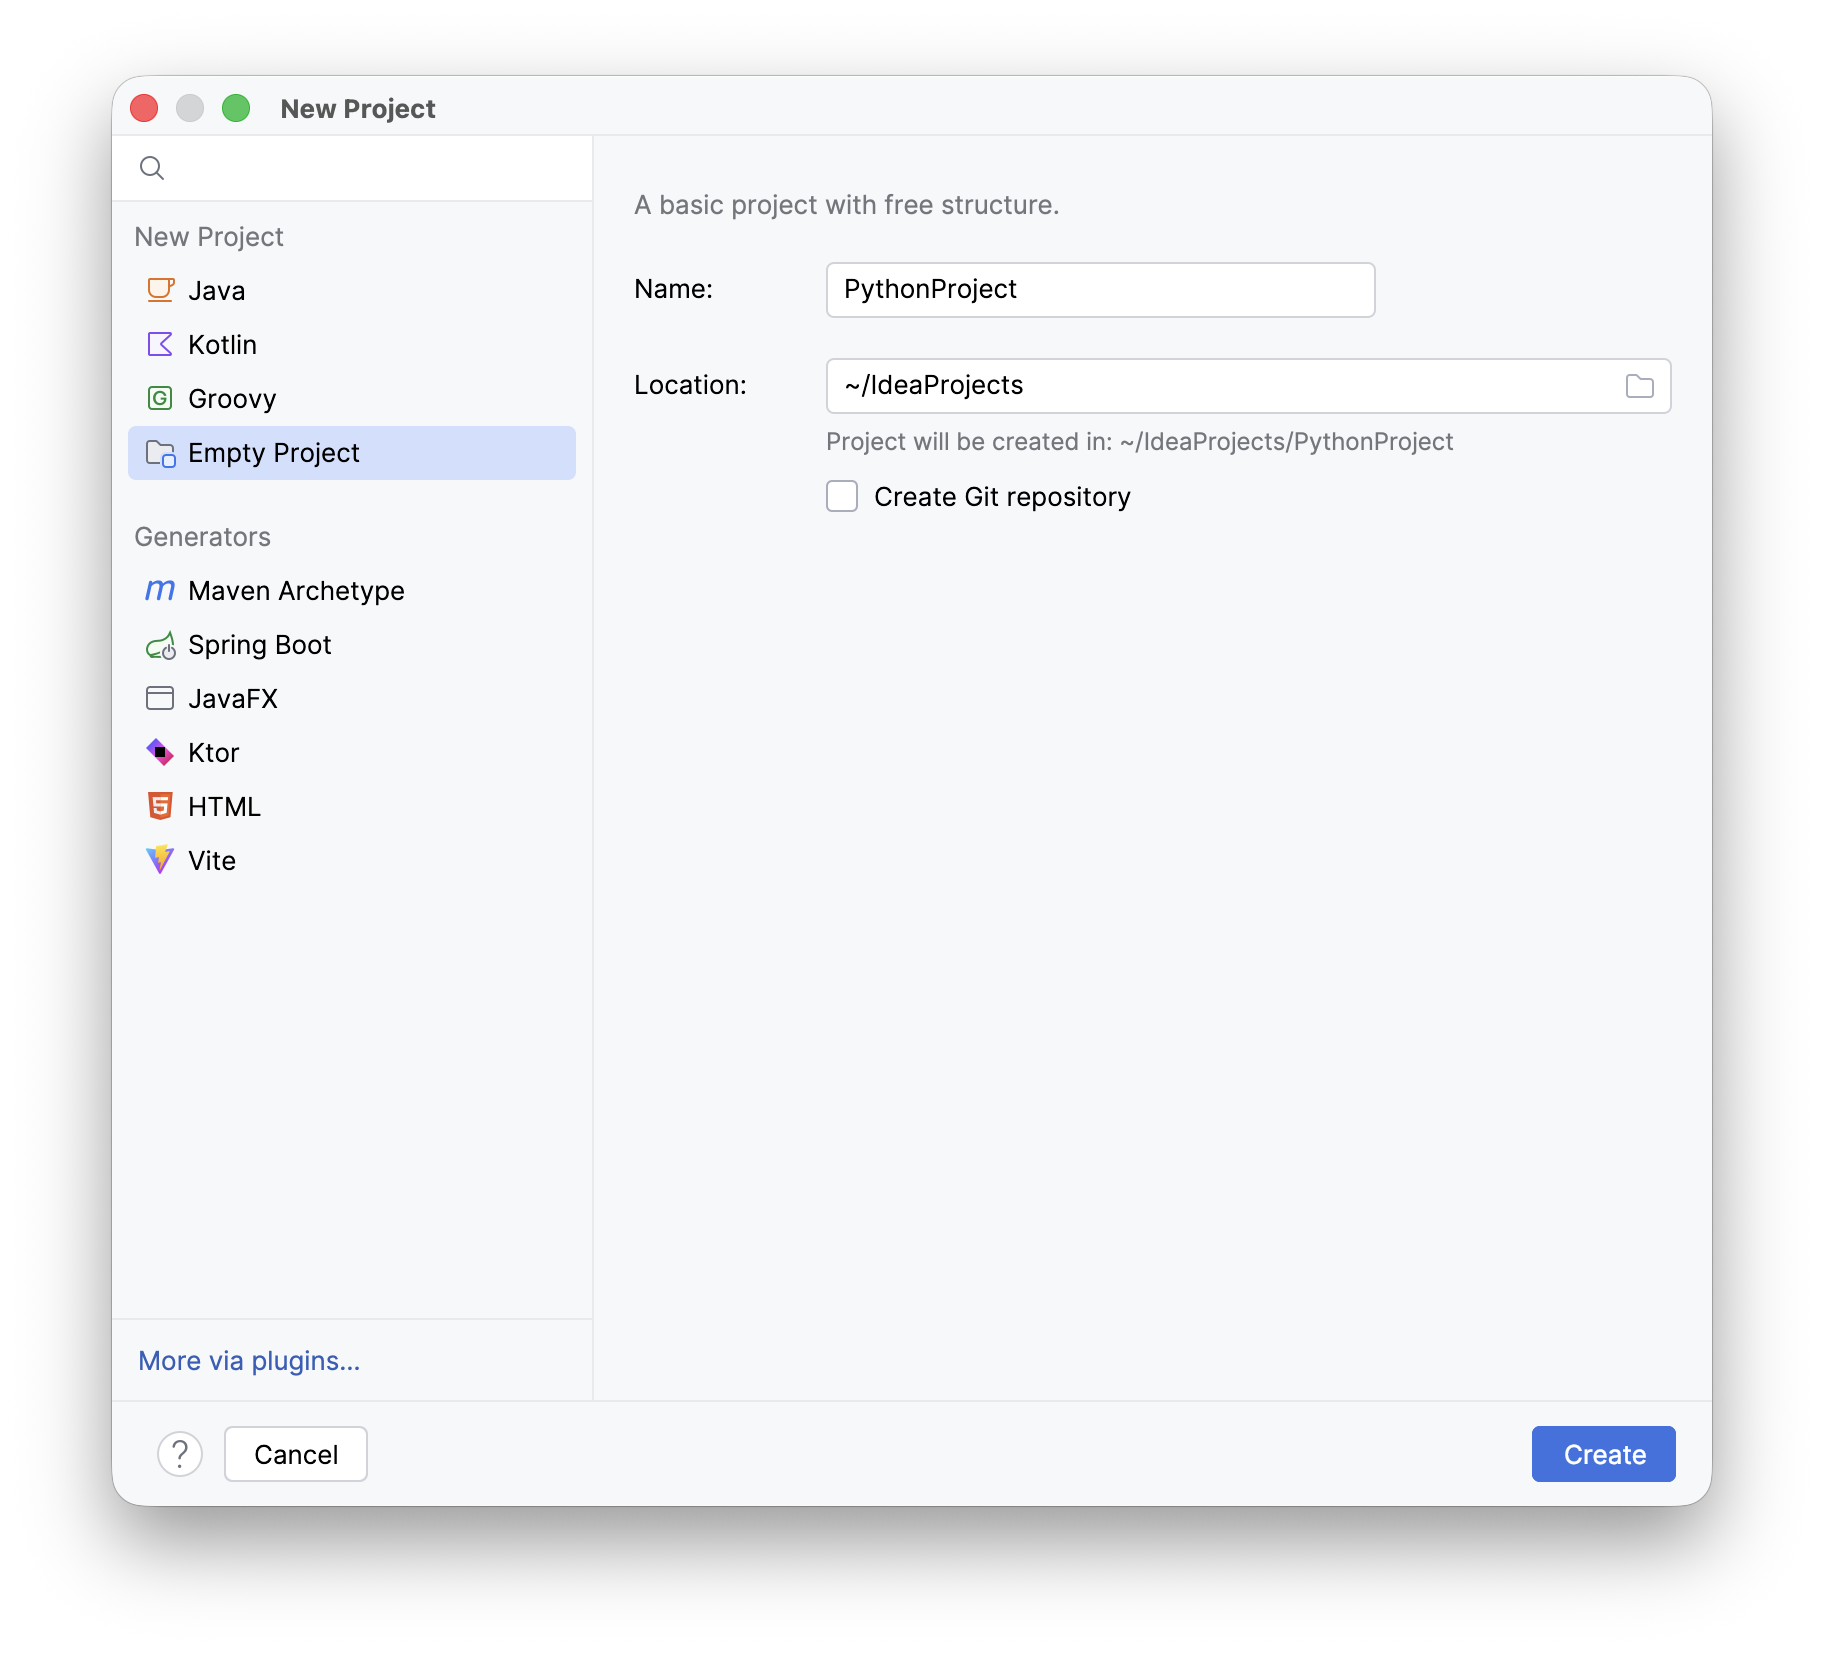
\includegraphics[width=\textwidth]{../img/macos/newproject.png}
        % Reproduce the open plugin menu shown over the old project screenshot.
        \par\vspace{-0.3\textwidth}
        \noindent\makebox[\textwidth][l]{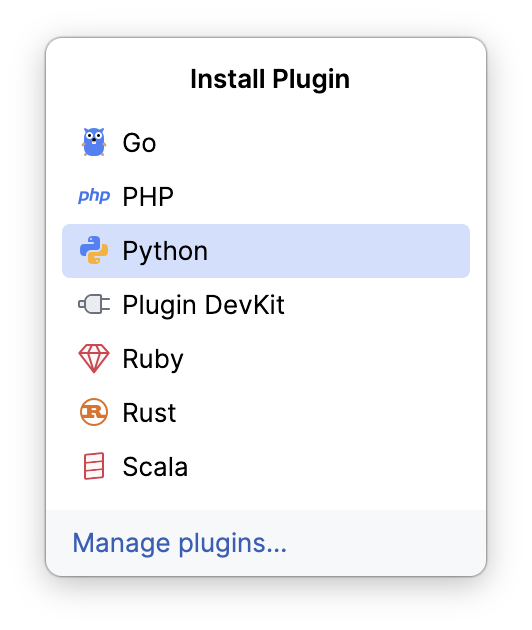
\includegraphics[width=0.38\textwidth]{../img/macos/pluginmenu.png}}
        \caption{Création d'un nouveau projet - Install Plugin}
        \label{fig:pluginmenu}
    \end{subfigure}
    \hfill
    \begin{subfigure}[t]{0.45\textwidth}
        \centering
        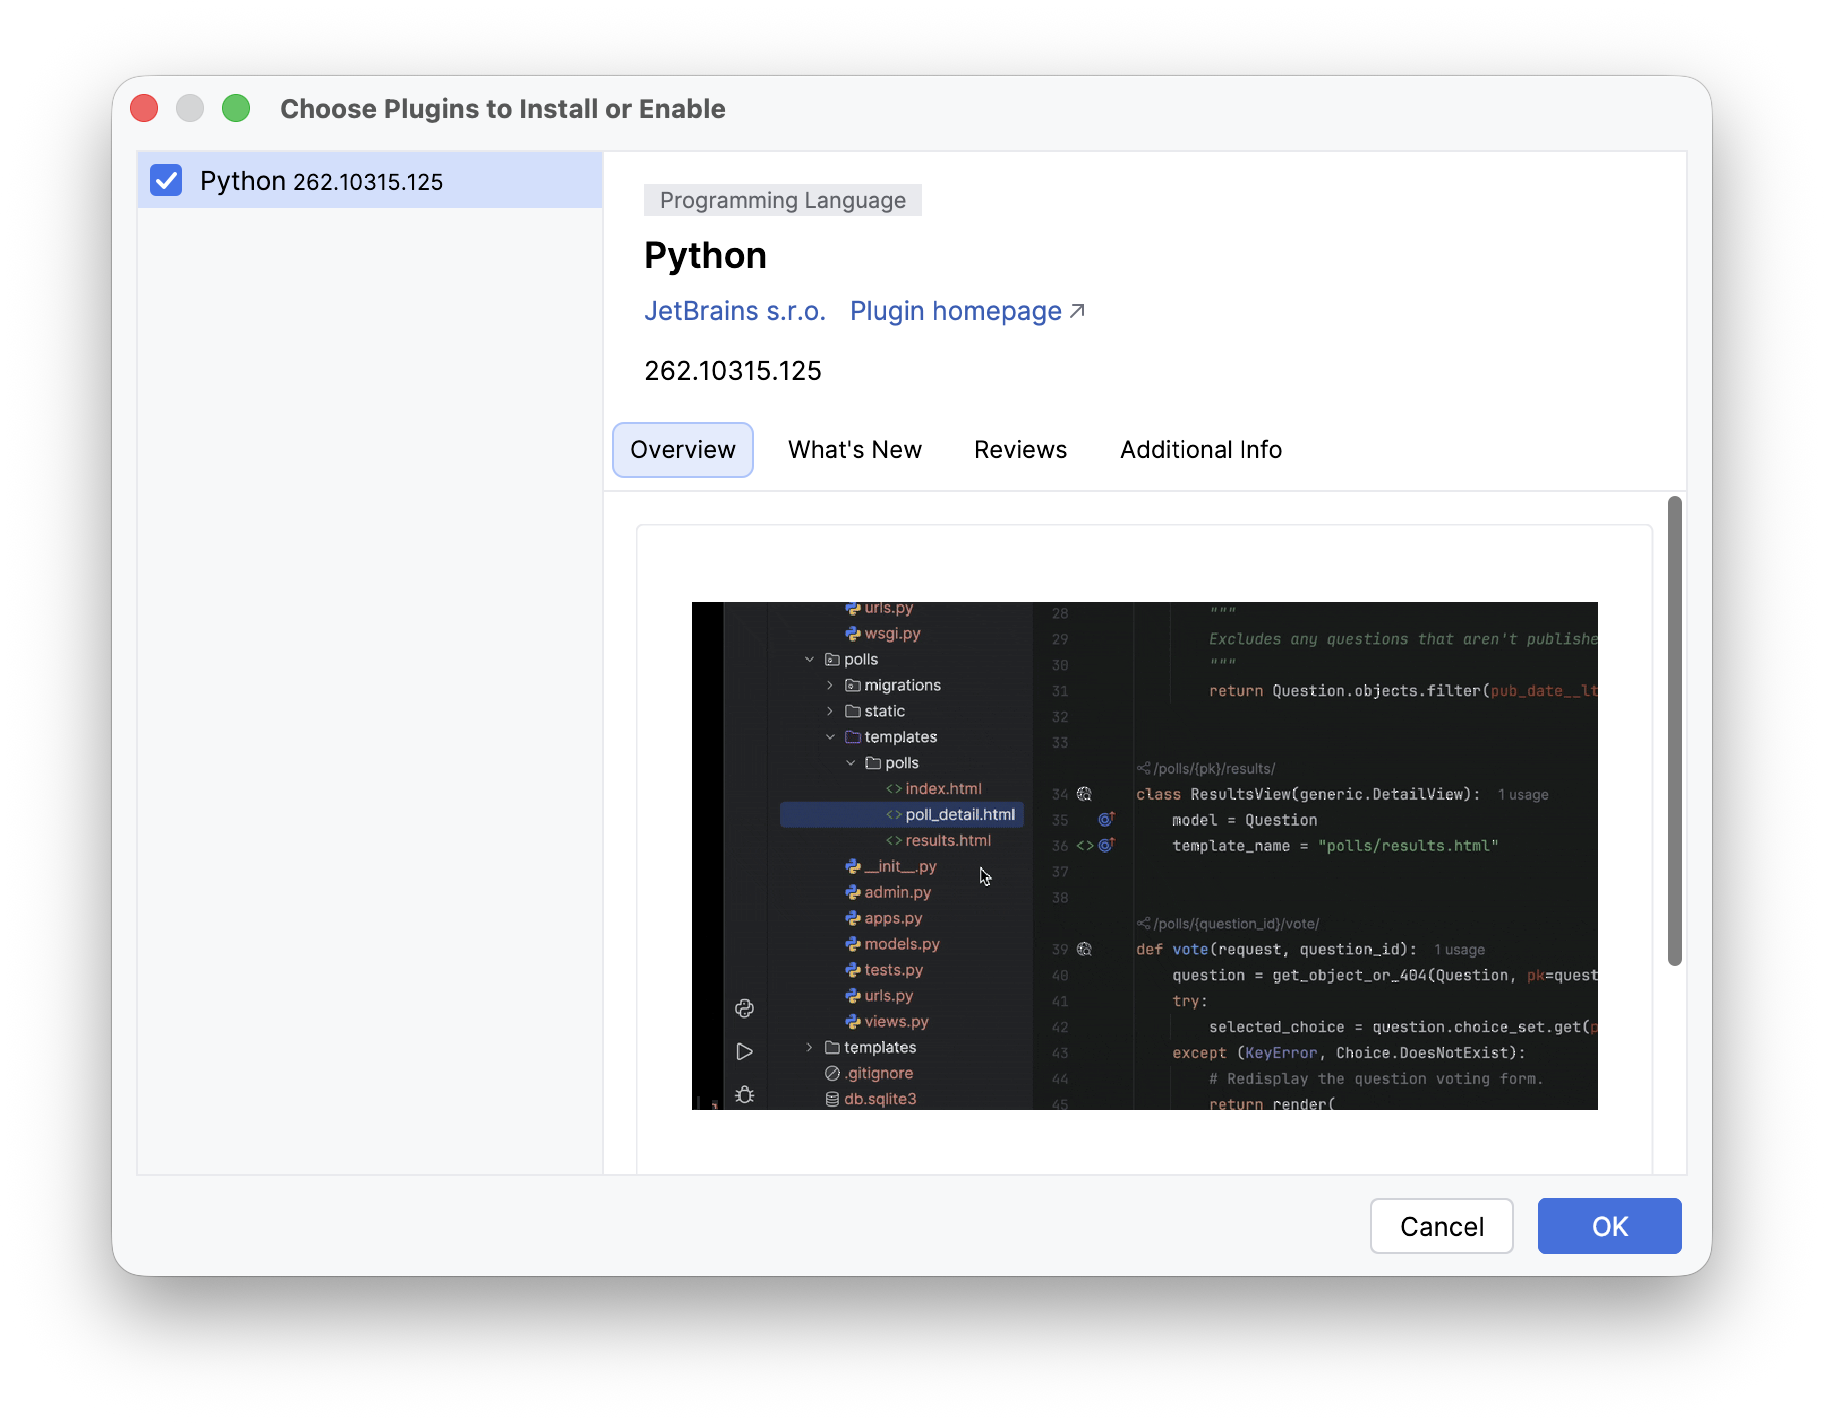
\includegraphics[width=\textwidth]{../img/macos/pluginpy.png}
        \caption{Installation du plugin Python}
        \label{fig:pluginpython}
    \end{subfigure}
    \caption{Utilisation de Python dans Intellij}
    \label{fig:installpython}
\end{figure}
    
    \item Pour créer un nouveau projet, cliquez sur \texttt{Create} à partir de la fenêtre d'accueil, sélectionnez Python ou Java sur le menu latéral à gauche. Définissez l'emplacement de votre kit de développement logiciel et donnez un nom à votre projet (Assurez-vous de choisir une version Python $>=$ 3.11). Cliquez sur \texttt{Create}.
    \begin{figure}[ht]
    \centering
    \begin{subfigure}[t]{0.45\textwidth}
        \centering
        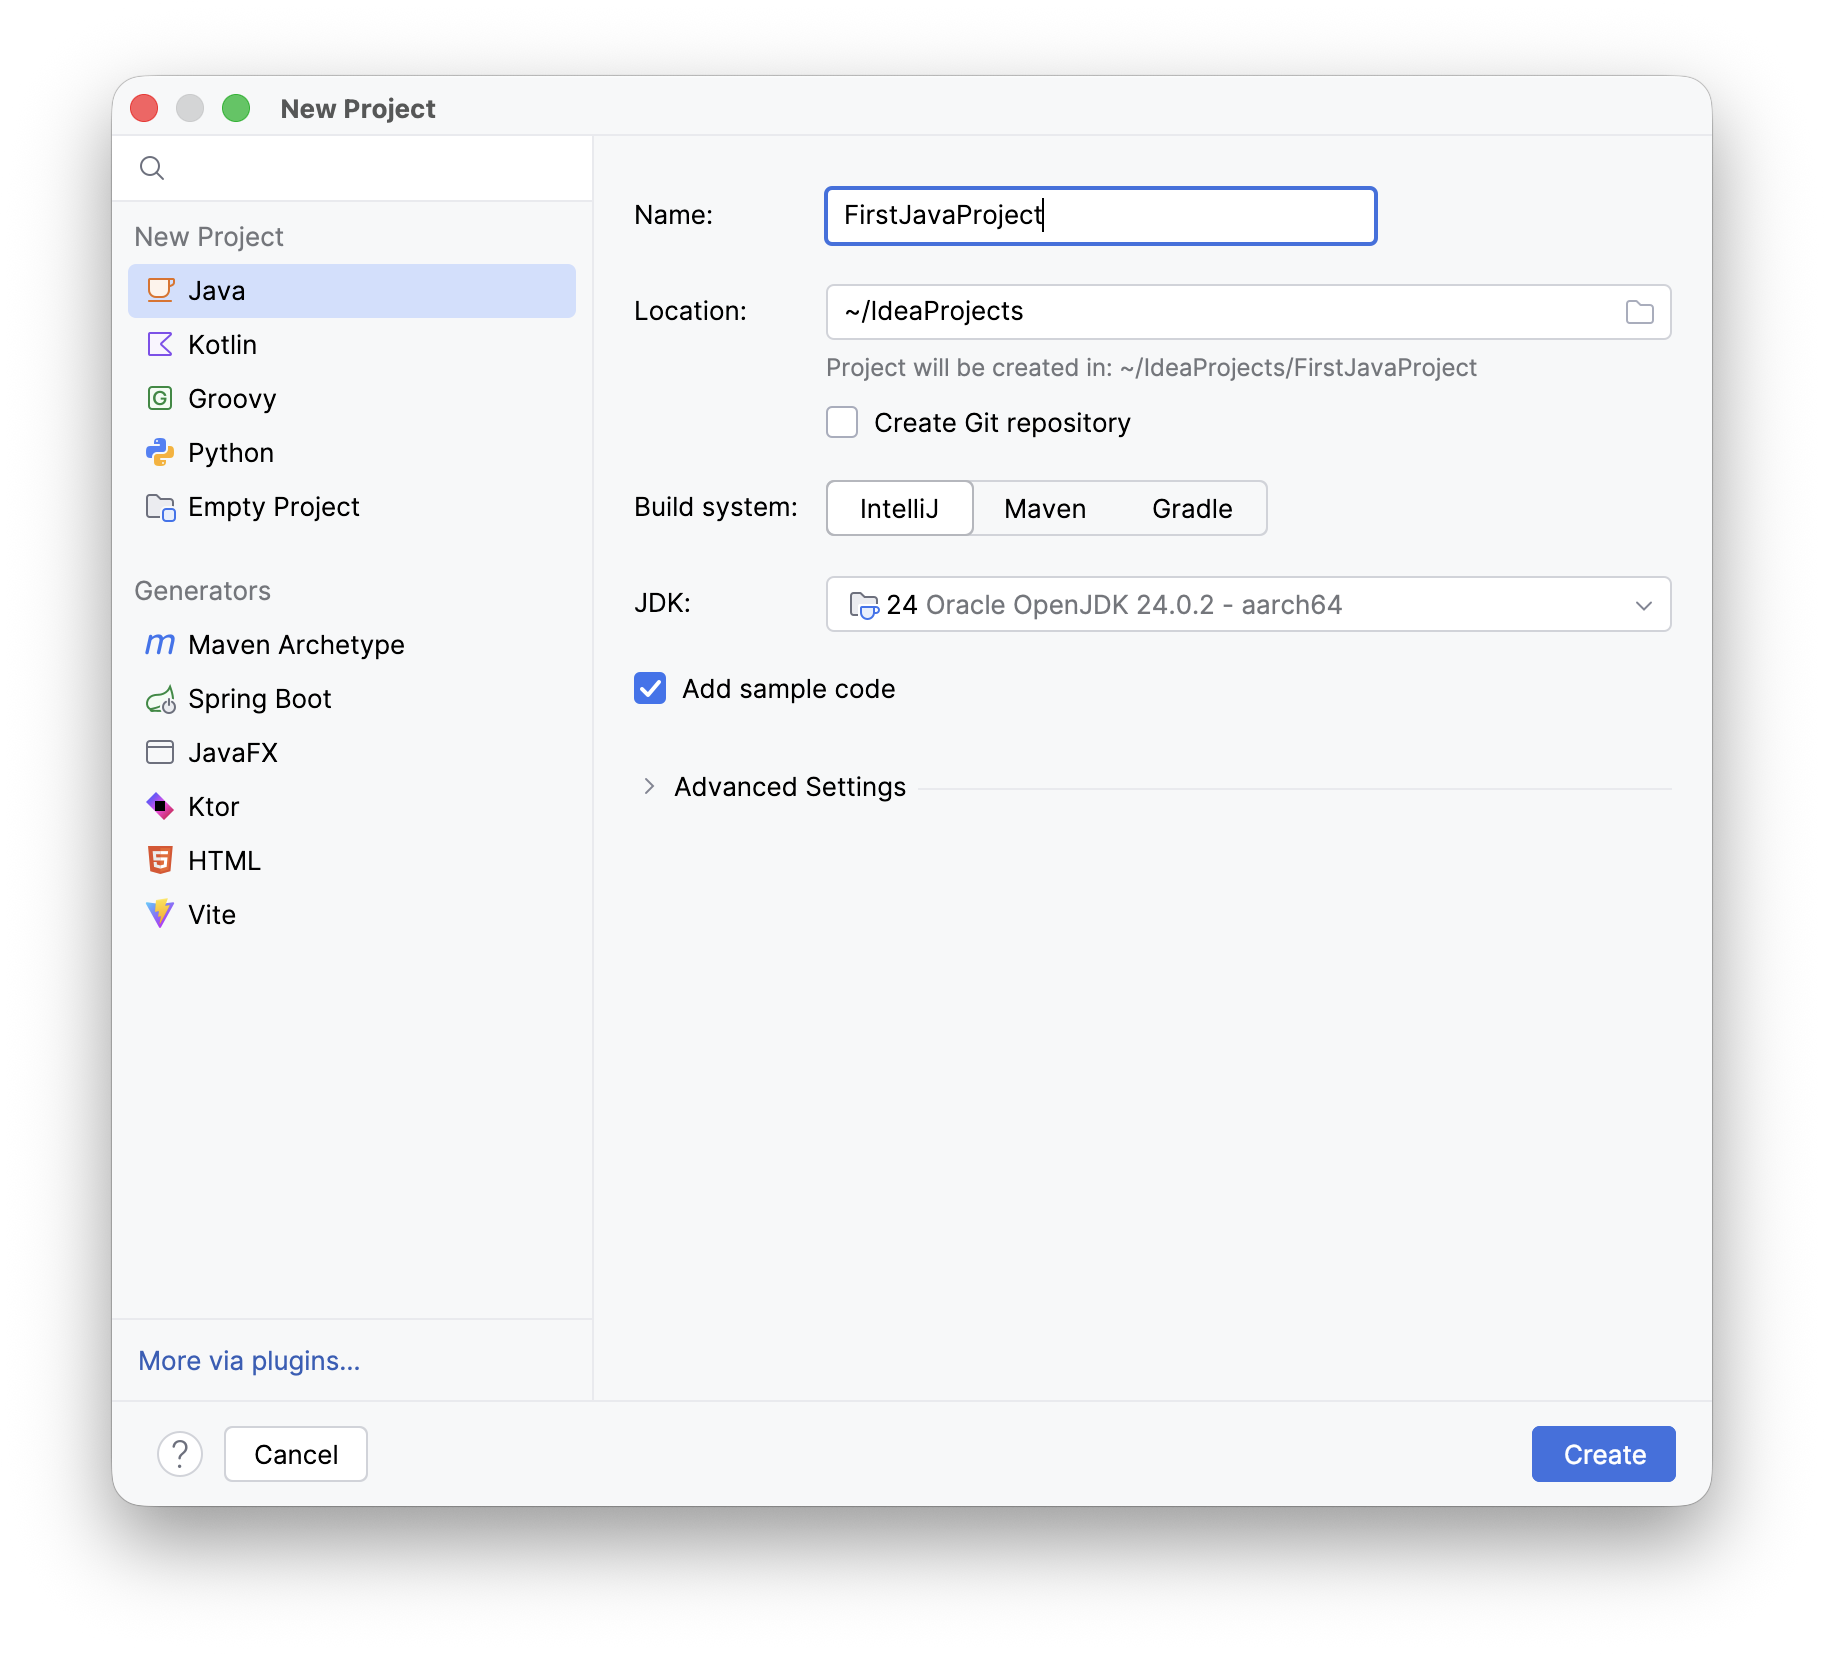
\includegraphics[width=\textwidth]{../img/macos/newprojectjava.png}
        \caption{Création d'un projet Java}
        \label{fig:sub1}
    \end{subfigure}
    \hfill
    \begin{subfigure}[t]{0.45\textwidth}
        \centering
        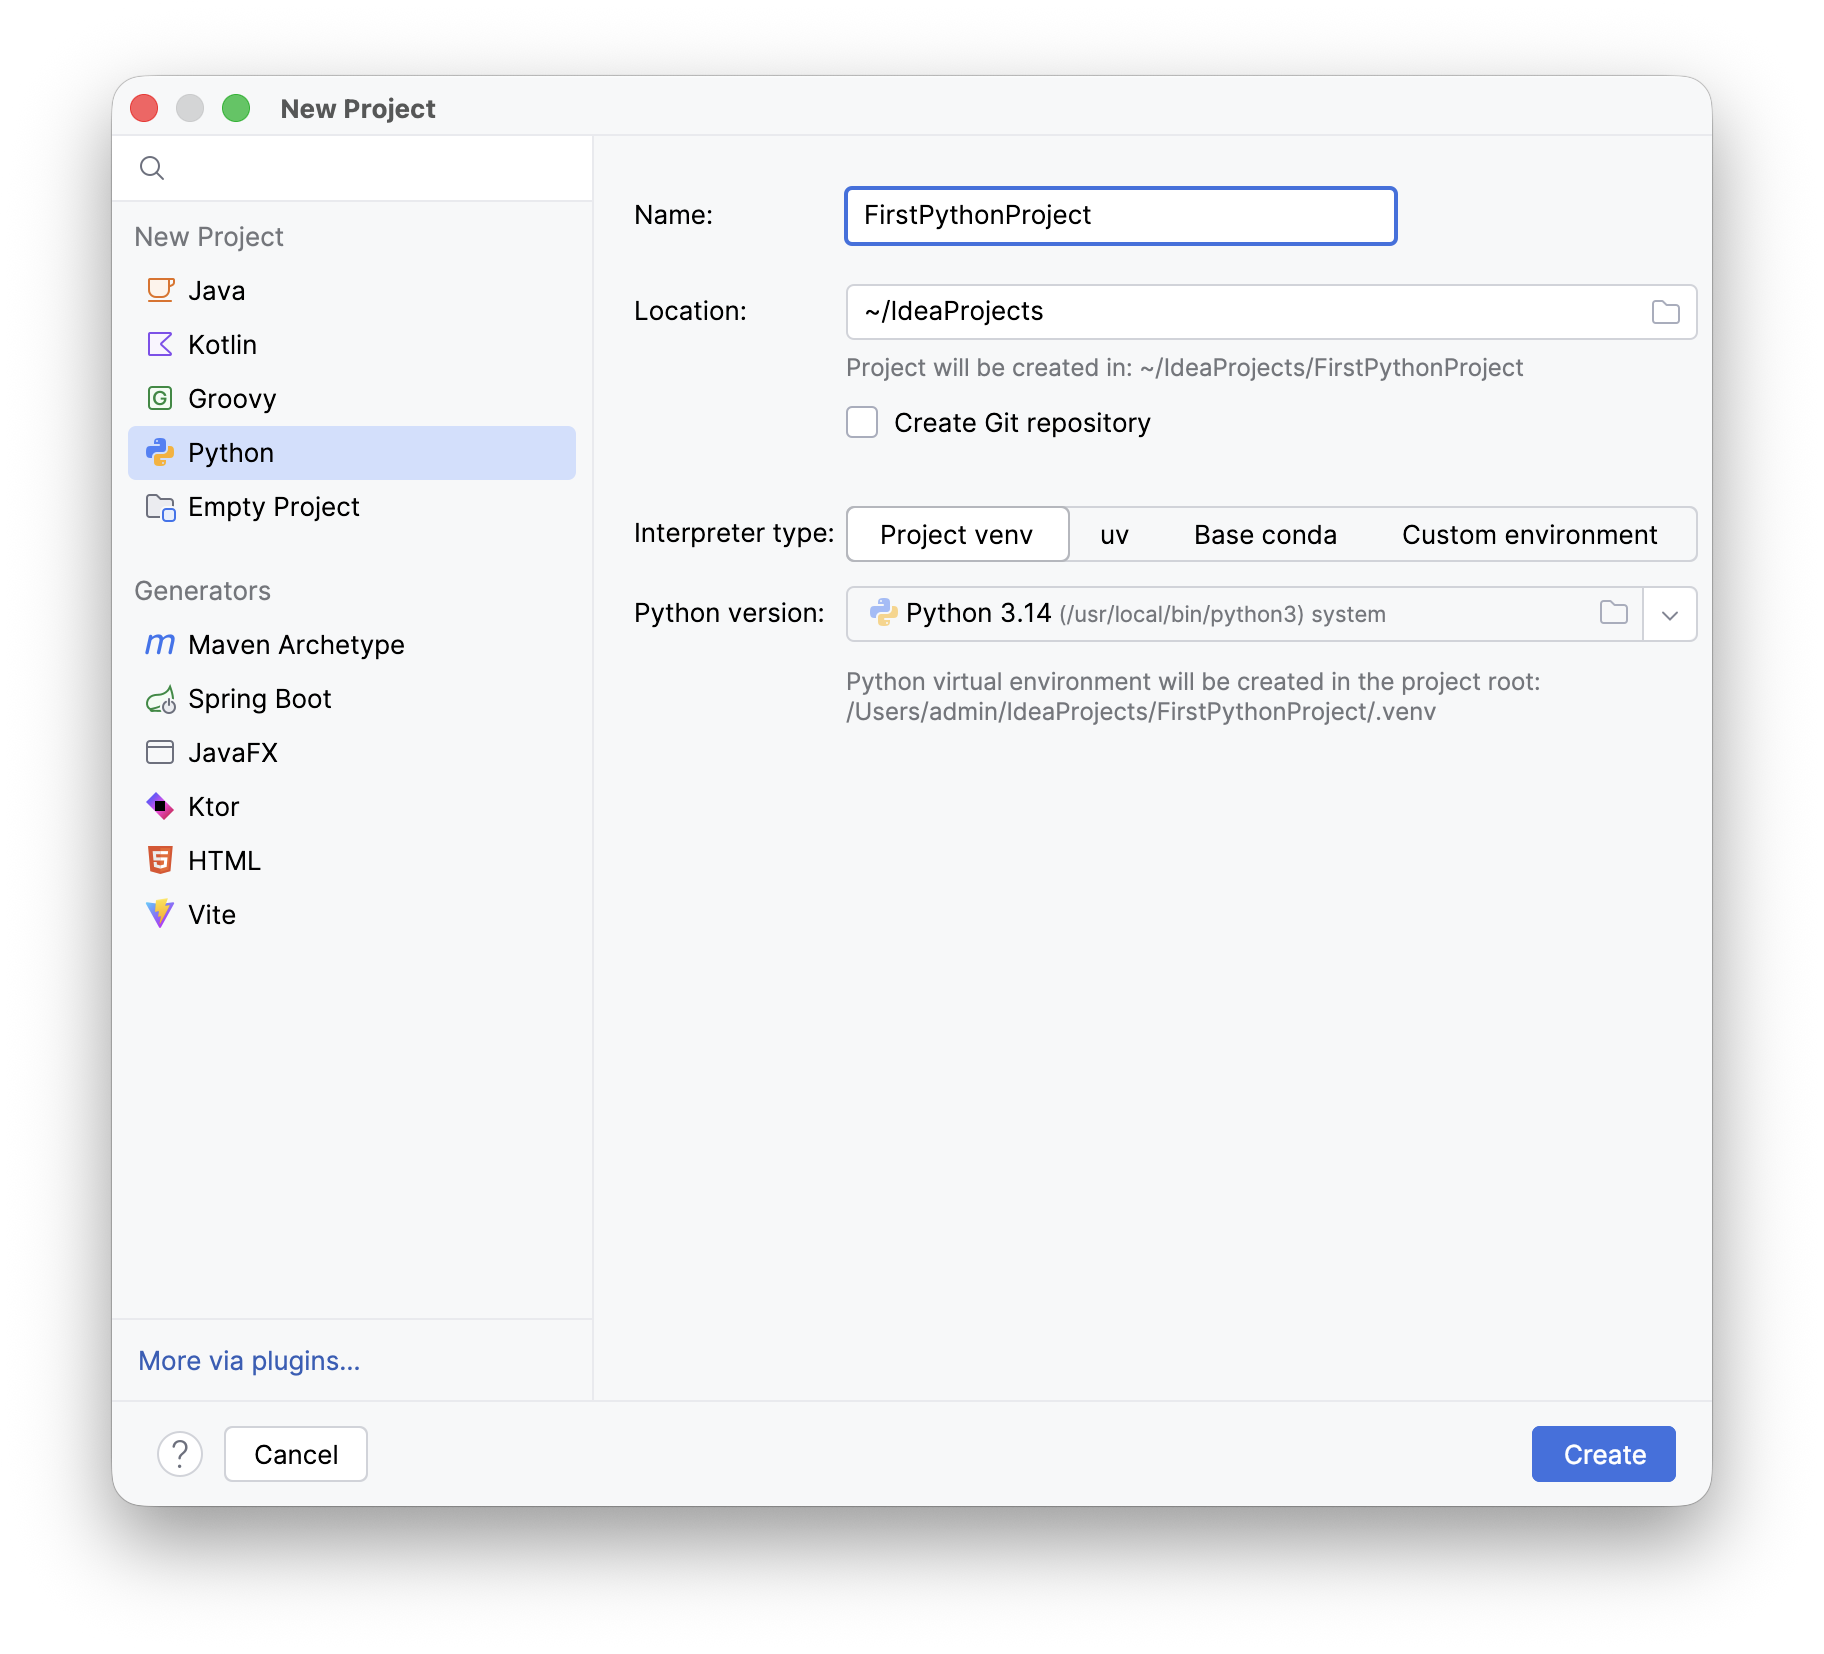
\includegraphics[width=\textwidth]{../img/macos/newprojectpy.png}
        \caption{Création d'un projet Python}
        \label{fig:sub2}
    \end{subfigure}
    \label{fig:createproject}
\end{figure}
\end{enumerate}
\newpage

\subsection*{Votre premier programme}

\begin{itemize}
    \item \textbf{Python: }\url{https://www.jetbrains.com/help/idea/creating-empty-python-project.html}
    \item \textbf{Java: }\burl{https://www.jetbrains.com/help/idea/creating-and-running-your-first-java-application.html#run_app}
\end{itemize}

\end{document}
